

\begin{frame}{Конвееры}
%  \textbf{Цель} -- максимальная модульность: большое количество простых приложений, взаимодействующих друг с другом для решения задач
  \only<1>{
  \begin{center}
    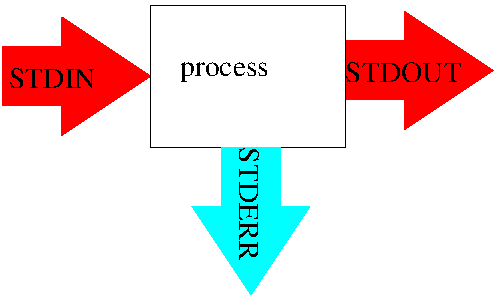
\includegraphics[width=1.2in]{../../slides/cmdline/process}
  \end{center}
  }
  \only<2>{
    \begin{center}
      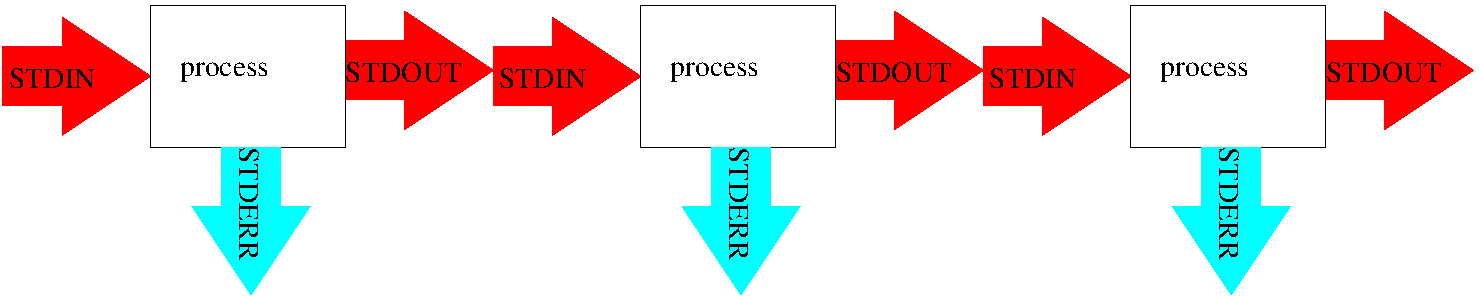
\includegraphics[width=3.6in]{../../slides/cmdline/processes}
    \end{center}
  }
  \begin{itemize}
    \item <1-> Каждое приложение открывает 3 стандартных файловых дескриптора stdin (fd 0), stdout(fd 1), stderr (fd 2)
    \item <2-> Приложения могут работать как фильтр из STDIN в STDOUT, можно объединять несколько приложений в конвейер
    \item <2-> Синтаксис {\tt <app1> | <app2>}
  \end{itemize}
\end{frame}
